\chapter{Background}

% keywords
\begin{itemize}
  \item BTOR2
  \item ANTLR
  \item Theta
  \item HWMCC
  \item XCFA
  \item model checking, formal verification
\end{itemize}

\section{Model Checking}
During the course of this project, I have familirized myself with the concept of model checking. 
Formal software verification uses mathematically precise proofs to verify the correctness of computer programs. Model checking is a widely used method that exhaustively checks every possible execution of a program for every possible input to see if certain properties are satisfied.
In my case, I focused mainly on reachability testing, which means we explore the state space of a program to see if a certain bad state can be reached.
In order to do this, we need to represent the program in a way that allows us to analyze its control flow and data flow. This is where the concept of control flow automata (CFA) comes into play.
\begin{figure}[h]
  \centering
  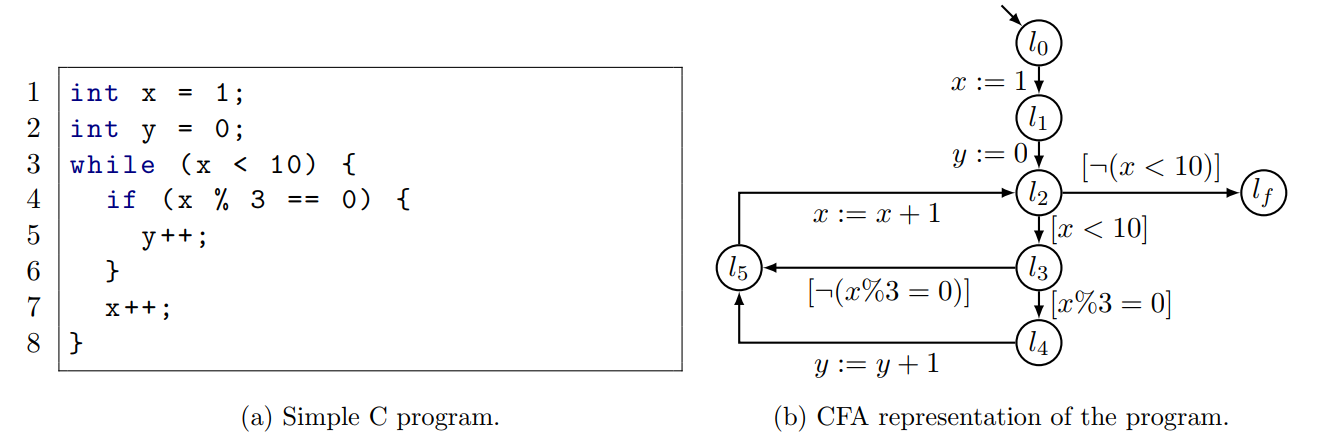
\includegraphics[width=0.5\textwidth]{figures/cfa_c.png}
  \caption{Simple C program and its corresponding control flow automaton (CFA).}
\end{figure}
In my documentation, I will describe how we can transform a BTOR2 program into a CFA and how we can use this representation to perform model checking.

\section{BTOR2}
The Hardware Model Checking Competition (HWMCC) serves as a benchmark for evaluating formal verification tools for hardware systems. A key innovation supporting this effort is BTOR2, a word-level model checking format designed for bit-precise modeling. Building on the earlier BTOR format, BTOR2 introduces a simple, sorted, line-based syntax that is easy to parse and aligns with SMT-LIB semantics for bit-vectors and arrays. It combines the low-level precision of formats like AIGER with higher-level abstractions, making it ideal for various verification techniques. 
\begin{figure}[h]
  \centering
  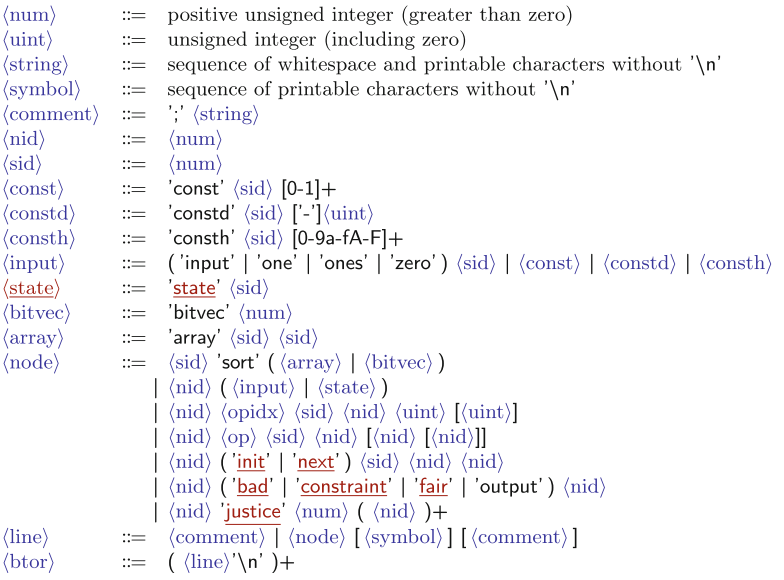
\includegraphics[width=0.5\textwidth]{figures/btor2_syntax.png}
  \caption{. Syntax of Btor2. Non-terminals opidx and op are indexed and non-indexed operators as defined in Table 1 (sequential part in red). (Color figure online)}
\end{figure}
\cite{btor2}
In my implementation I focused on bit vectors and its related functions and definitions.

\section{ANTLR}
We have written an unofficial BTOR2 grammar format using ANTLR4.
ANTLR (ANother Tool for Language Recognition) is a powerful parser generator widely used in both academia and industry to build interpreters, compilers, and DSLs. Based on LL parsing, it reads grammar files and automatically generates lexers and parsers for multiple languages, including Java, C++, and Python. ANTLR cleanly separates syntax from application logic using *listener* and *visitor* patterns, enabling maintainable and modular code.
This makes ANTLR an excellent tool for writing a BTOR2 grammar, as its clear structure, support for complex syntax rules, and language flexibility make it easy to build robust parsers for BTOR2's line-based, sorted format.
\cite{antlr}
% TODO: szépíteni

\section{Theta}
My main goal was to achieve a BTOR2 frontend for the Theta model checker.
Theta is a modular and extensible model checking framework developed by the Critical Systems Research Group at the Budapest University of Technology and Economics. It is designed to support a wide range of verification techniques, particularly abstraction refinement-based reachability analysis, and is capable of analyzing various low-level formalisms such as Control Flow Automata (CFA), Symbolic Transition Systems (STS), and Timed Automata.
One of Theta's major strengths is its support for high-level frontends, allowing users to model complex systems in languages like C or UML statecharts, which are then automatically translated into formal representations. This makes Theta highly accessible and adaptable for both research and practical applications.
In my project, I used XCFA models, an extension of CFA that includes support for procedures and concurrency, but I focused specifically on the CFA parts, applying Theta's powerful CEGAR-based algorithms for reachability checking.
\cite{theta}